\subsubsection{Face recognition and human tracking}
\subsubsection{Object recoginition and manipulation}
Tinker uses a two-phase approach to recognize target and precisely manipulate them. In the first phase, a point cloud is built from the kinect v2 depth camera. Hough transform and an entropy-based filter is applied to the point cloud to remove the backgroud. Then a euclidean clustering is employed to give the region of interest. A typical image of the filtered point cloud is given below:
\begin{figure}[H]
    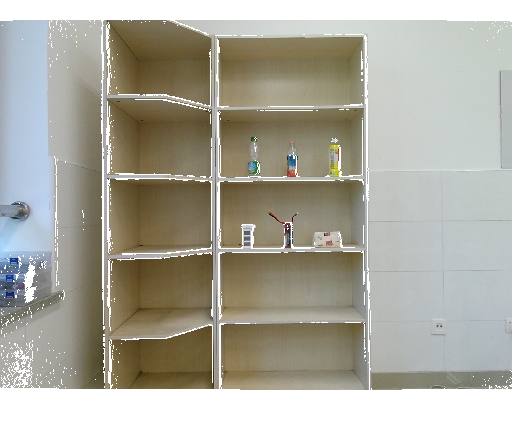
\includegraphics[scale=0.5]{original.png}
    \caption{original image}
\end{figure}

\begin{figure}[H]
    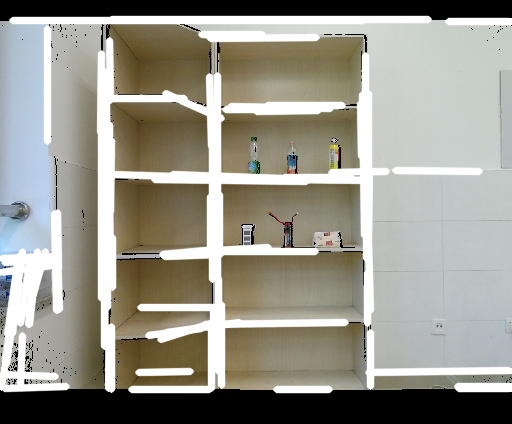
\includegraphics[scale=0.5]{filtered.png}
    \caption{filtered image}
\end{figure}

In the second phase, the approximate location of object is given to the robot arm controller, another usb camera placed in the hand of the robot arm will guide the arm to precisely manipulate the object. First, the hand is moved to directly face the location of the region of interest at about 40 cm away. A similar image processing pipeline is used to find the object in the image given by the camera in hand. After getting the image of the object, it is matched with the pre-captured image set by convolution the image with the templates to find the best mattch. Precision of the location found in this phase is significantly improved due to a much closer camera place. Then the robot arm will be guided by the camera using a feedback procedure to place the object in the middle of the camera image. Thus, the chance of missing the object is reduced.

